%\documentclass[a4paper,10pt]{jarticle}
%\documentclass[]{jarticle}
\documentclass[10pt]{jsarticle}

%\usepackage{graphicx}
\usepackage[dvipdfmx]{graphicx}
\usepackage{eclbkbox} %breakbox用
\usepackage[T1]{fontenc}
\usepackage{lmodern}
\usepackage{amsmath}
\usepackage{ascmac} %shedebox用
\usepackage{here} %図を好きな位置に
\usepackage{here}
\usepackage{listings, jlisting}
\usepackage{framed}

\lstset{%
  language={c},%言語名前
  basicstyle={\footnotesize\ttfamily},%ソースコードのフォント設定
  identifierstyle={\small},
  ndkeywordstyle={\small},
  keywordstyle={\ttfamily},
  stringstyle={\small\ttfamily},
  frame={tb},
  breaklines=true,%行が長くなった際の改行の有無
  xrightmargin=0zw,%右の余白の大きさ
  xleftmargin=3zw,%左の余白の大きさ
  numbers=left,%行番号表示場所
  stepnumber=1,%行番号の増分
  numbersep=1zw,%行番号と本文の間隔
  numberstyle=\ttfamily,
  frame=tRBl,
  framesep=5pt,
  commentstyle={\ttfamily},%コメントアウトのフォント設定
  flexiblecolumns = true,
  classoffset=1,
  showstringspaces=false,
  tabsize=4
}


%本文領域を広め(空白箇所マージン領域を小さめ)に設定
\setlength{\textwidth}{179mm}
\setlength{\textheight}{251mm}
\setlength{\topmargin}{-2cm}
\setlength{\oddsidemargin}{-1cm}
\setlength{\evensidemargin}{-1cm}

\begin{document}

\title{情報工学実験IIレポート(探索アルゴリズム2)}
\author{曜日&グループ番号: 金曜&グループ9} %
\date{\today}

\maketitle


\section*{グループメンバ}
今回は実験は全体で行ったが,レポートは分担して作業した.
以下にレポート作成時の分担を示す.

\begin{itemize}
 \item 155706J 久場翔悟: 担当Level2
 \item 155711E 平木宏空: 担当Level1
 \item 155716F 石塚海斗: 担当Level3.1,3.4
 \item 155730B 清水隆博: 担当Level3.2,3.3
\end{itemize}

\section*{提出したレポート一式について}
レポート一式は
\verb|``naha:/home/home/teacher/tnal/jikken1-fri/e945734/''|
にアップロードした。
提出したファイルのディレクトリ構成は以下の通りである。\\
\begin{breakbox}
\begin{verbatim}
./src/      # 作成したプログラム一式
./report/   # レポート関係ファイル.図ファイルを含む.
\end{verbatim}
\end{breakbox}

\newpage

\section{Level1: 線形分離可能なOR問題への適用}
\subsection{課題説明}
2入力1出力で構成される単純パーセプトロン(ニューラルネットワーク)を
用いて、
4つの教師信号を用意したOR問題へ適用し、
重みが適切に学習可能であることを確認する。
また、学習が収束する様子をグラフとして示す。

 %課題説明
\subsection{OR問題を学習させた際の誤差収束度合いについて}
\subsubsection{実験結果}
NNでは重みを更新する毎に誤差が減るように学習を行うが、その学習の様子は初期の重みを設定している乱数シード値を1000から100刻みに,10000万まで変更し,実行した.
シード値を変えた際の学習収束回数を表\ref{table:level1}に示す。
シード値を10回変更して学習させた際の重みを更新する様子を図
\ref{fig:level1-1}に、
その平均をプロットした平均推移値を図\ref{fig:level1-2}に示す。


\begin{table}[htb]
 \begin{center}
  \caption{OR問題の学習に要した回数}
  \label{table:level1}
  \begin{tabular}[htb]{r|l} \hline
   シード値 & 収束した回数 \\ \hline \hline
   100 & 96 \\ \hline
   200 & 90 \\ \hline
   300 & 111 \\ \hline
   400 & 109 \\ \hline
   500 & 93 \\ \hline
   600 & 99 \\ \hline
   700 & 100 \\ \hline
   800 & 114 \\ \hline
   900 & 113 \\ \hline
   1000 & 94 \\ \hline \hline
   10試行の平均値 & 101.9 \\ \hline
  \end{tabular}
 \end{center}
\end{table}




\begin{figure}[h]
 \begin{center}
  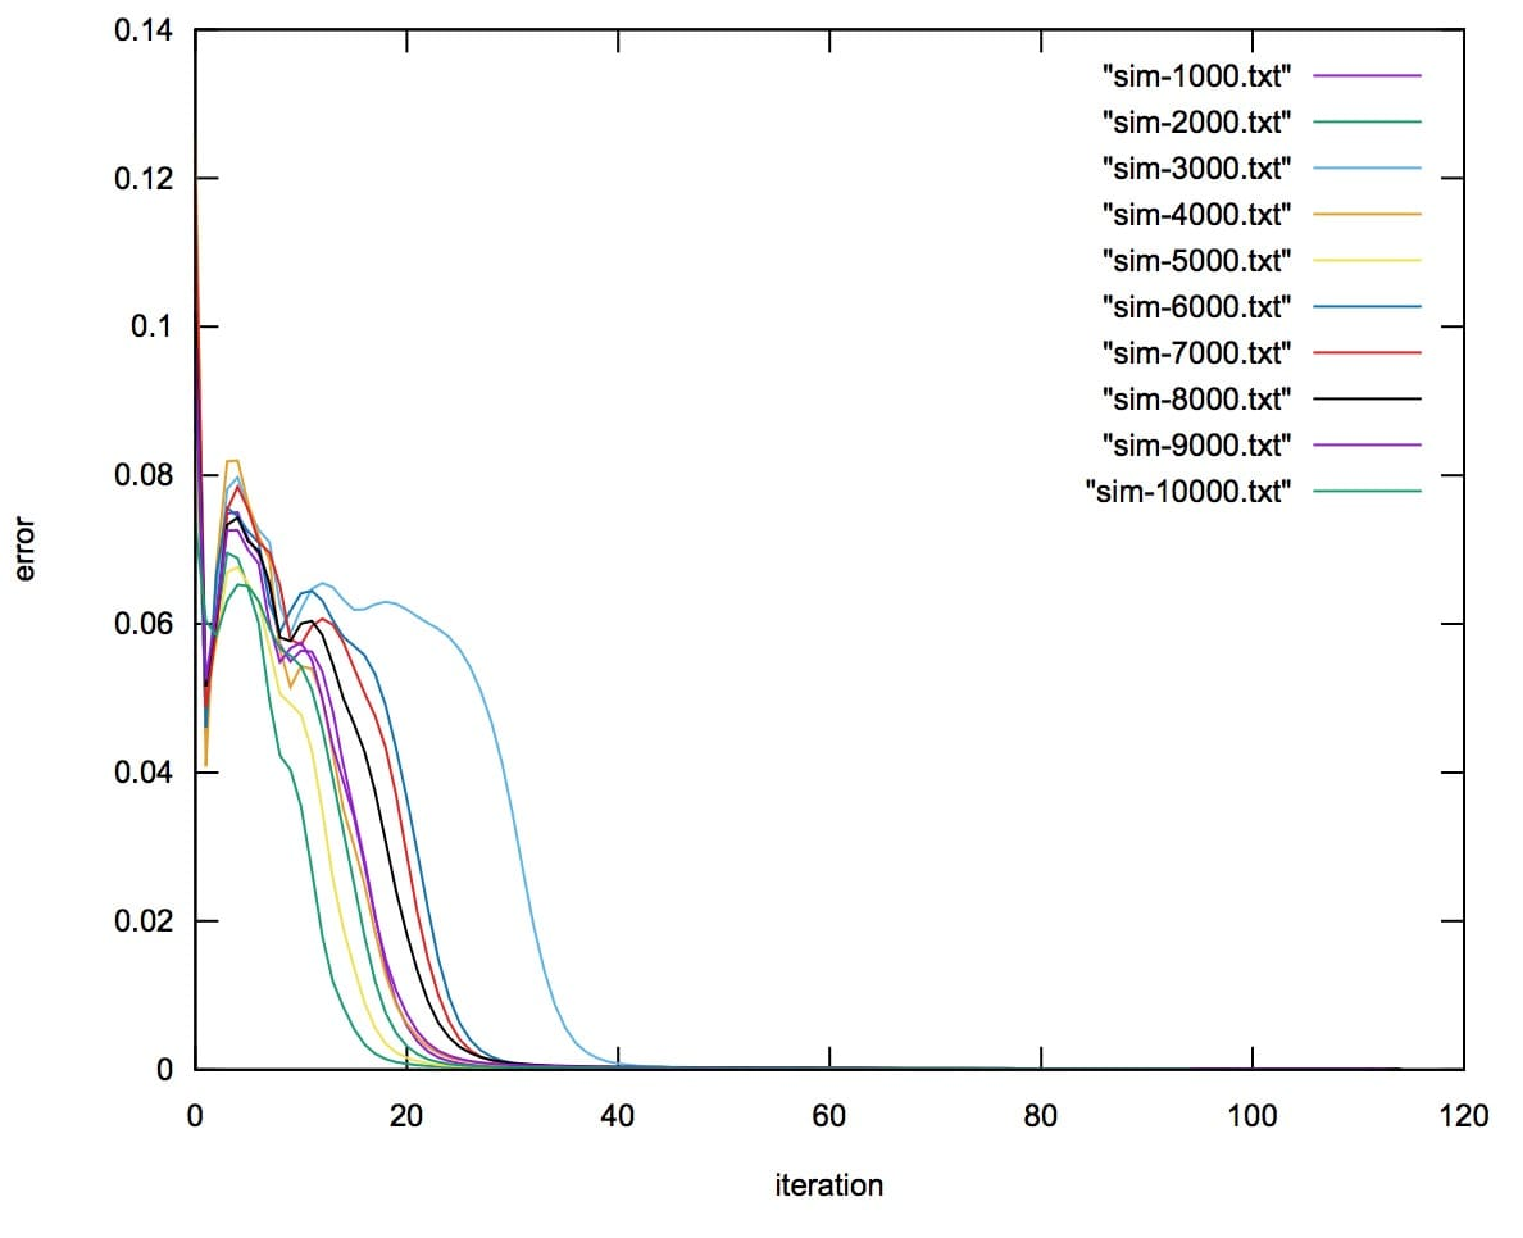
\includegraphics[width=10.0cm]{figs/seeds.pdf}
  \caption{重みを更新する様子}
  \label{fig:level1-1}
 \end{center}
\end{figure}

\begin{figure}[h]
 \begin{center}
  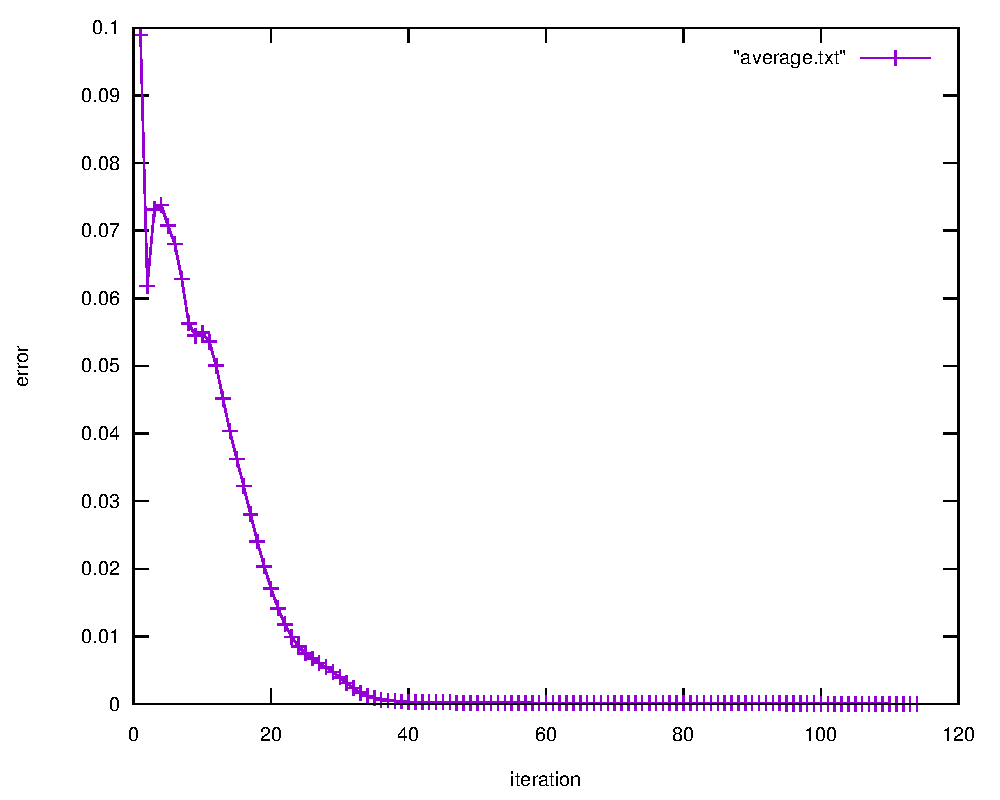
\includegraphics[width=10.0cm]{figs/average.pdf}
  \caption{重みを更新する様子(平均値)}
  \label{fig:level1-2}
 \end{center}
\end{figure}


\subsubsection{考察}
実行結果よりシード値(重み)に関わらず,100回前後の学習でほぼ誤差が0に限りなく近くなることがわかった.

\subsection{「OR問題」を学習させた際の学習の推移(iteration vs error)をグラフ化し、そのグラフ化手順と共に示せ。}

以下のシェルスクリプトも用いて,実験を行った.グラフ作成にはgnuplotを使用した.
\lstinputlisting{./seed.sh}
\lstinputlisting{./sum.sh}
\lstinputlisting{./average.sh}








\newpage

\section{Level2: 線形分離不可能なExOR問題への適用}
\subsection{課題説明}
階層型ニューラルネットワークをExOR問題へ適用し、
線形分離できない問題においても学習可能であることを確認する。
特にLevel2では、
この問題を解決するために中間層を導入することで拡張した階層型ニューラルネッ
トワークにより学習可能であることを確認する。



 %共通部分の結果及び考察
\subsection{階層型NNによる学習}
\subsubsection{最適なパラメータを探すためのアプローチ}
指定された条件下において学習が効率良く行われるパラメータの組み合わせを探
すため、**して**することでパラメータを調整した。

(補足:全パターンを調べても良いし、いくつかのパターンを調べても良いが、
どのような方法で調整したら良いかを考えよう)


\subsubsection{実行結果}

(補足:シード値10パターンで試した際の収束に要した学習回数と、その平均回数が分かるように明示してください。)
\begin{table}[htb]
 \begin{center}
  \caption{階層型NNによるExOR問題の学習に要した回数}
  \label{table:level2}
  \begin{tabular}[htb]{r|l} \hline
   シード値 & 収束した回数 \\ \hline \hline
   100 & hoge \\ \hline
   200 & hoge \\ \hline
   300 & hoge \\ \hline
   400 & hoge \\ \hline
   500 & hoge \\ \hline
   600 & hoge \\ \hline
   700 & hoge \\ \hline
   800 & hoge \\ \hline
   900 & hoge \\ \hline
   1000 & hoge \\ \hline \hline
   10試行の平均値 & hoge \\ \hline
  \end{tabular}
 \end{center}
\end{table}

\begin{figure}[h]
 \begin{center}
  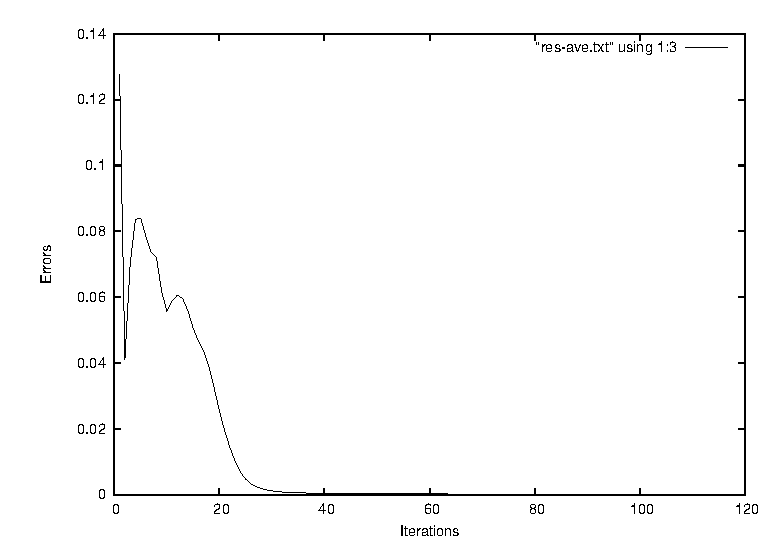
\includegraphics[width=10.0cm]{figs/sample2.eps}
  \caption{重みを更新する様子(平均値)}
  \label{fig:level2}
 \end{center}
\end{figure}


\subsubsection{考察}



\newpage

\section{Level3: 応用事例:文字認識問題への適用}
\subsection{課題説明}
階層型NNを文字認識に適用し、考察する。
特に、用意された教師データと認識のしやすさに関する関係性や、
学習最適化のためのパラメータのチューニングおよび、
より柔軟性の高い認識方法に関する検討を行う。

 %課題説明
\subsection{Level3.1: パラメータのチューニング}
\subsubsection{最適なパラメータを探すためのアプローチ}
指定された条件下において学習が効率良く行われるパラメータの組み合わせを探
すため、**して**することでパラメータを調整した。

(補足:全パターンを調べても良いし、いくつかのパターンを調べても良いが、
どのような方法で調整したら良いかを考えよう。その上で、自分たちがどのよ
うに取り組んだのか(=アプローチ)を説明しよう。)

\subsubsection{実行結果}

(補足:ボーナスポイントの確認がありますので、シード値10パターンで試した際の収
束に要した学習回数と、その平均回数が分かるように明示してください。)
\begin{table}[htb]
 \begin{center}
  \caption{階層型NNによる文字認識問題の学習に要した回数}
  \label{table:level3}
  \begin{tabular}[htb]{r|l} \hline
   シード値 & 収束した回数 \\ \hline \hline
   100 & hoge \\ \hline
   200 & hoge \\ \hline
   300 & hoge \\ \hline
   400 & hoge \\ \hline
   500 & hoge \\ \hline
   600 & hoge \\ \hline
   700 & hoge \\ \hline
   800 & hoge \\ \hline
   900 & hoge \\ \hline
   1000 & hoge \\ \hline \hline
   10試行の平均値 & hoge \\ \hline
  \end{tabular}
 \end{center}
\end{table}

\begin{figure}[h]
 \begin{center}
  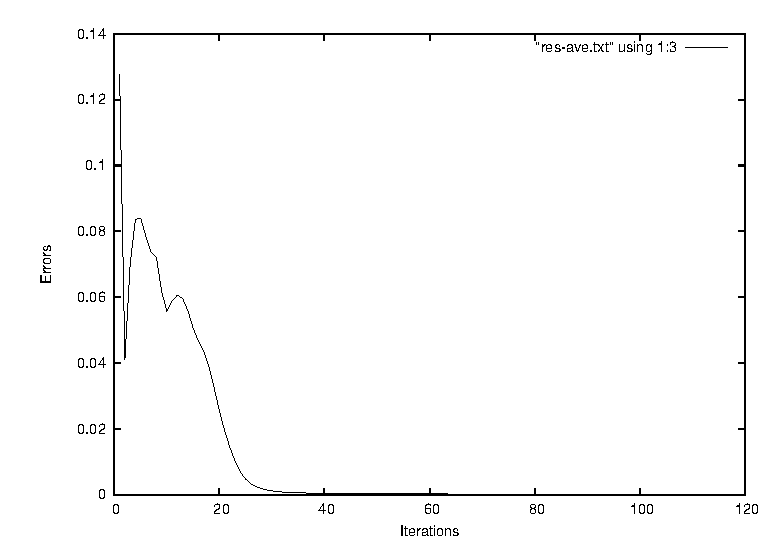
\includegraphics[width=10.0cm]{figs/sample2.eps}
  \caption{重みを更新する様子(平均値)}
  \label{fig:level2}
 \end{center}
\end{figure}


\subsubsection{考察}



\subsection{Level3.2: パラメータと収束能力の関連性について}
\subsubsection{関係性を確認するためのアプローチ}
文字認識プログラムnn\_numではいくつかのパラメーターが設定されているが,今回はETA,ALPHA,HIDDENに着目する.
これらパラメーターが収縮能力にどのような影響を及ぼすのかを今回は考察する.
尚,起動時にはもう1つパラメーターとしてseed値を入力する必要がある.
しかし今回のプログラムではseedはあまり関係が無く学習が収束する.
従って今回の検証ではseed値は1000に固定を行った.

\subsubsection{実際の検証について}
今回実際に検証するに対して,前述の3種類のパラメーターの影響を考察する.
方法としては確認対象のパラメーターを変動させ,それ以外のパラメーターを固定した状態で実際に学習を行う.
この出力結果を比較し,それぞれがどの様な影響を及ぼすかを調査した.
Level3.1では幾つかのパターンで総当りを行ったが,今回の実験では実際にこれら全てのデータは使用しない.
それぞれのパラメーターに対して,実行した数値から3つ選び,実行した.
実行結果から比較を行い,今回は合計9回学習を行っている.

探索では幾つかのシェルスクリプト.及びグラフのplotにgnuplotを用いた.

今回検証したパターンを示す.


\begin{itemize}
    \item ALPHA 0.50 HIDDEN 5に設定
        \begin{itemize}
        \item ETA 0.01 の場合
        \item ETA 1.00 の場合
        \item ETA 1.98 の場合
        \end{itemize}
    \item ETA 1.50 HIDDEN 5に設定
        \begin{itemize}
            \item ALPHA 0.01 の場合
            \item ALPHA 1.00 の場合
            \item ALPHA 1.98 の場合
        \end{itemize}
    \item ALPHA 0.50 ETA 1.0に設定
        \begin{itemize}
            \item HIDDEN 1 の場合
            \item HIDDEN 5 の場合
            \item HIDDEN 15 の場合
        \end{itemize}

\end{itemize}

今回収縮能力を考察するにあたり,run\_nn.bashを一部改良し利用した. 変更部分をdiffコマンドを用いて表す. (ソースコード:\ref{nnbashr})
\lstinputlisting[caption=run\_nn.bashの変更点,label=nnbashr]{nnbash.diff}
主な変更点は,タイトルの表示を今回変更したパラメーターに対応させ,seed値を1000で固定した.
また\LaTeX でレポートを作成する際にPDF形式が編集し易い為,出力形式をpdfに変更した.

今回はこのスクリプトと,nn\_num内で実行する処理を記述したcommand2.txtを用いて動作させた.
以下に今回実行したコマンド例を示す.
\begin{oframed}\begin{verbatim}
$bash nn_num "HIDDEN5" < command2.txt
      \end{verbatim}
\end{oframed}

尚パラメーターの変更は,自動化するべきであったが,手動でヘッダーファイルを編集し都度makeを実行した.

\subsubsection{結果}

まずETAを変更した場合の実行結果を示す. (図:\ref{fig:ETAresult})
処理の段階で,先程のbashスクリプトで一つずつのグラフを作成している.
しかし,今回はパラメーターを変更した場合の比較を確認したい為,各条件で処理を実行した後に纏めてグラフ化を行った.
グラフ化にはシェルスクリプトを用いたが,各処理はおおよそ共通している.
その為,今回レポートで示すシェルスクリプトは一つとする. (ソースコード:\ref{gnuplotALPHA})

\lstinputlisting[caption=gnuplotALPHA.sh,label=gnuplotALPHA]{../nn/nn_num/src/gnuplotALPHA.sh}

今回はplotしたいテキストファイル名が既に確定していた為,静的にスクリプト内に記述している.
もし大規模な実験データをplotする場合,ある一定の命名規則に則ったテキストファイルをplotするような記述に
変更するべきであると考える.
また,gnuplotでpdf出力を選択した場合replotを繰り返すと同一pdfファイル内にreplotした時点での画像データが
新しいページとして保存される.
今回はまとめたデータのみ必要だった為,全てreplotした後に出力先をpdfに変更しreplotしている.

\begin{figure}[H]
    \centering
    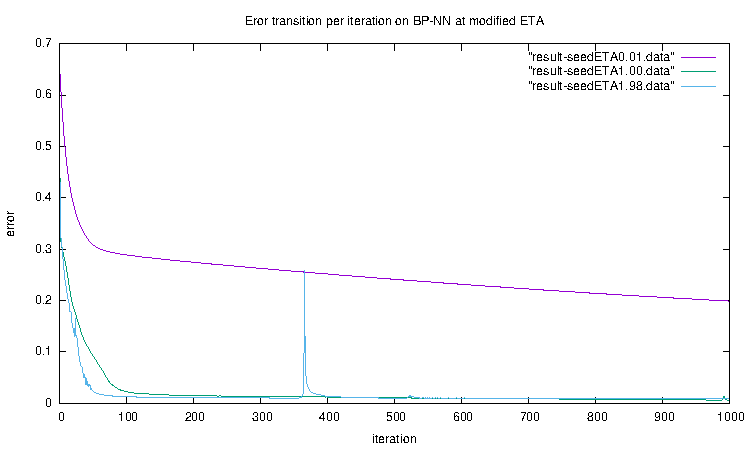
\includegraphics[width=0.8\textwidth]{figs/Level3.2/ETA.pdf}
    \caption{ETAの値を変更した場合の推移}
\label{fig:ETAresult}
\end{figure}

グラフを確認すると,ETAの値が大きくなるに連れてerrorの数値が減少している事が読み取れる.
また,共通して初回のerrorが大きく,iterationの回数が増えていくにつれてerrorが減少していく.
ETA1.98の場合,300から400の間で一度極端にerrorの値が上昇しているが,これは必ずしもerrorが改善されないことに起因していると推測する.
この実家から,ETAに関してはなるべく大きな数値で実行するとerrorの発生を抑えられることが判断出来る.

続いてALPHAの値を変更した場合の挙動を確認する. (図:\ref{fig:ALPHAresult})

\begin{figure}[H]
    \centering
    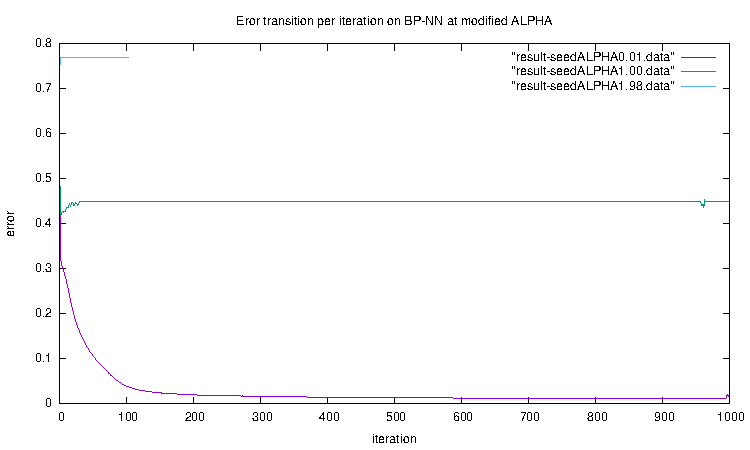
\includegraphics[width=0.8\textwidth]{figs/Level3.2/ALPHA.pdf}
    \caption{ALPHAの値を変更した場合の推移}
\label{fig:ALPHAresult}
\end{figure}

この図を確認すると,ALPHAの値が0.01の場合,errorがiterationを重ねるに連れて減少していくことが読み取れる.
しかし,ALPHAの値を1.0にした場合は,むしろ初回よりerrorが上昇した.
さらにiteration 100以降の場合はほとんどerrorの値に変化が見られなかった.
1.98の場合はiteration100を超えた場合,正常にerrorの結果がプログラムから取得出来なかった.
従って,慣性項ALPHAに関しては今回の結果から考察すると0に近い数値にするとより良く収束する.
また,数値を大きく取ってしまうと,正常に実験が出来ないと推測する.

最後にHIDDENの値を変化させた場合の挙動を確認する. (図:\ref{fig:HIDDENresult})

\begin{figure}[H]
    \centering
    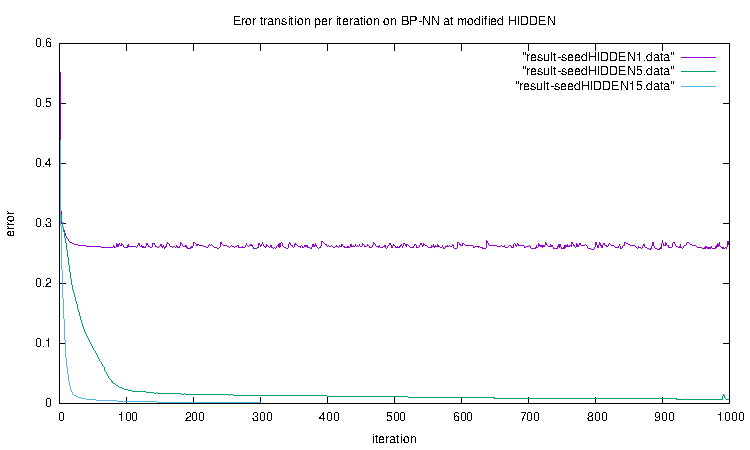
\includegraphics[width=0.8\textwidth]{figs/Level3.2/HIDDEN.pdf}
    \caption{HIDDENの値を変更した場合の推移}
\label{fig:HIDDENresult}
\end{figure}

実行結果からHIDDENの値を1にした場合,微少に上限に変動し続けるが,おおよそerrorが一定の値を保つ事がわかる.
しかし,5,15にHIDDENの値を設定した場合,iteration 100までで急激にerrorが低下し,以降は一定という挙動を示した.
さらにHIDDENを15にした場合,他の2種類よりiterationの回数が圧倒的に低かった.

\subsubsection{考察}
今回の実行結果を確認するとETAの値は1.98,ALPHAが0.01,HIDDENが15の場合それぞれ良い収束結果を見せた.
中間層ユニットHIDDENの数は学習結果を集約させしすぎてしまうと捨てられるデータが大きくなると推測する.
しかし,ある一定サイズより多く確保しても入力データそのものに対して違いが無い為,最終的なerrorの値は同様になると考える.

学習係数ETAは最急降下法と同じく探索点を更新する際の動きを制御するパラメーターである.
この値は小さい場合精度が上がると考えられるが,今回の場合iterationの収束を考えると1以上の大きさの値にするべきであると考察する.

慣性項は今回の場合,極力小さな値で実行するべきであると考える.
慣性の通り,前回の探索点との変化を示す\cite{sizuoka} 為,大きすぎると探索点の移動に支障が出てしまうと考える.
特に1.00にした場合ほとんど動かなかった.
以上のことよりこれらパラメーターを最適値にする場合,ある程度職人技のような微調整が必要であると考える.

\subsection{Level3.3: 任意の評価用データを用いた評価}

level3.3では文字認識プログラムnn\_numにおいて,評価用データが教師用データと異なる場合,認識結果に違いが見られるかを実験する.

\subsubsection{アプローチ}
実験を行うにあたり,学習用データと評価用データがずれていくにあたり,認識率がどう変動するか仮説を検討した.
文字認識の場合,計算機に学習させるアルゴリズムによって最終的な認識に至るまでのプロセスが異なると考える.しかし,あくまで認識は学習用データを利用し行う.
教師あり学習の場合,明確な答えが定義されている学習用データそのものが入力された場合の認識率は最大であると考える.
また,今回の実験で使用した文字認識プログラムは0か1の数値データに基づいて学習を行う.
人間では誤差の範囲であるが,計算機の場合1bitの変化で計算した内容が大幅に変化していくのではないかと推測した.
従って,学習用データからずれていくに連れて文字を誤認識する確率が上昇するのではないかとの仮説を立てた.

この仮説のもと,「二,三,五」の3種類の数字に着目し,いくつか差分を作成し認識率の変化を測定した.

\subsubsection{実験内容}
作成したデータはそれぞれ漢数字の「二,三,五」を少しずつ変更したものである.
これら3文字はそれぞれ横線が多く,五に関しては横線と斜め,及び縦線で構成されている.
例えば三という文字の二画目の横棒に「払い」の様な記述を加えると五だと認識されるのではないか.
また,二の払いを横棒と認識出来るレベルにまでいれると,一,もしくは三として判断されるのではないかとも考えた.
従って,構成している要素が英数字よりも単純な漢数字の3つで今回は測定を行う.

差分データを作成する場合,機械的に変更するべきであると考える.
しかし今回は文字認識であり,実際には手書き文字などの判断につながっていく分野である.
その為,人間が想定できる範囲の変更を手動で行い,機械的にランダムに変更するアプローチは取らなかった.
しかし,3種類の文字とは言え実験データを用意するのは手間である.
今回はその問題を解決するために,引数に応じて教師用データを10個のテキストファイルへとコピーするシェルスクリプトを作成した.
実際に使用したスクリプトを示す. (ソースコード:\ref{makeeval})
\lstinputlisting[caption=makeeval.sh,label=makeeval]{../nn/nn_num/src/data.level3.3/makeeval.sh}

それ以降の文字の変更は前述の通り手動で行った.

実際に作成したデータは
\begin{oframed}
\begin{verbatim}
./nn/nn_num/src/data.level3.3
\end{verbatim}
\end{oframed}
ディレクトリ下に保存している.

命名規則はそれぞれ,evel [2,3,5]- [0-9]+.txtである.

\subsubsection{変更したデータ群}
今回変更したデータ群を示す.
ただし全件記述すると3*10=30個のデータを記述することになる.
レポートの体裁上,多く記載しすぎても問題があると判断し,今回はそれぞれ3つずつの記載に留めた. (ソースコード:\ref{eval22} $\sim$ \ref{eval510} )
作成したデータは全てディレクトリ内に保存しているので参照されたい.

\begin{figure}[H]
    \begin{center}
        \begin{tabular}{c}

            \begin{minipage}{0.33\hsize}
                \begin{center}
                \lstinputlisting[caption=eval2-1.txt,label=eval21]{../nn/nn_num/src/data.level3.3/eval2-1.txt}
                \end{center}
                \end{minipage}

                \begin{minipage}{0.33\hsize}
                    \begin{center}
                        \lstinputlisting[caption=eval2-3.txt,label=eval23]{../nn/nn_num/src/data.level3.3/eval2-3.txt}
                    \end{center}
                    \end{minipage}
                \begin{minipage}{0.33\hsize}
                    \begin{center}
                        \lstinputlisting[caption=eval2-5.txt,label=eval25]{../nn/nn_num/src/data.level3.3/eval2-5.txt}
                    \end{center}
                    \end{minipage}
        \end{tabular}
\end{center}
\end{figure}

\begin{figure}[H]
    \begin{center}
        \begin{tabular}{c}

            \begin{minipage}{0.33\hsize}
                \begin{center}
                \lstinputlisting[caption=eval3-3.txt,label=eval33]{../nn/nn_num/src/data.level3.3/eval3-3.txt}
                \end{center}
                \end{minipage}

                \begin{minipage}{0.33\hsize}
                    \begin{center}
                        \lstinputlisting[caption=eval3-5.txt,label=eval35]{../nn/nn_num/src/data.level3.3/eval3-5.txt}
                    \end{center}
                    \end{minipage}
                \begin{minipage}{0.33\hsize}
                    \begin{center}
                        \lstinputlisting[caption=eval3-10.txt,label=eval310]{../nn/nn_num/src/data.level3.3/eval3-10.txt}
                    \end{center}
                    \end{minipage}
        \end{tabular}
\end{center}
\end{figure}

\begin{figure}[H]
    \begin{center}
        \begin{tabular}{c}

            \begin{minipage}{0.33\hsize}
                \begin{center}
                \lstinputlisting[caption=eval5-3.txt,label=eval53]{../nn/nn_num/src/data.level3.3/eval5-3.txt}
                \end{center}
                \end{minipage}

                \begin{minipage}{0.33\hsize}
                    \begin{center}
                        \lstinputlisting[caption=eval5-5.txt,label=eval55]{../nn/nn_num/src/data.level3.3/eval5-5.txt}
                    \end{center}
                    \end{minipage}
                \begin{minipage}{0.33\hsize}
                    \begin{center}
                        \lstinputlisting[caption=eval5-10.txt,label=eval510]{../nn/nn_num/src/data.level3.3/eval5-10.txt}
                    \end{center}
                    \end{minipage}
        \end{tabular}
\end{center}
\end{figure}

\subsubsection{結果}
今回実験を行うにあたり,最終的な評価の出力のみ抽出したい.
またテキストファイル化し結果を保存したいので,シェルスクリプトを用いて自動で実験及び結果の抽出を行った.
今回作成し実行したシェルスクリプトを示す. (ソースコード:\ref{searchlevel23})

\lstinputlisting[caption=search\_level2.3.sh,label=searchlevel23]{../nn/nn_num/src/search_level2.3.sh}

このシェルスクリプトではまずdata.level3.3ディレクトリ内のresultがファイル名に含まれるtxtファイルを削除する.
その後ディレクトリ中の評価用テキストファイルを1つずつfor文で変数fileにパスを代入しながら処理を行う.
for文中では,nn\_numを起動する.今回はseed値を1000に固定し3回学習をした後にcheckを行い,fileを評価する.
nn\_numでの一連の処理の結果は一次ファイル.tmpに保存し,得たい評価結果のみcutとsedを用いて切り出す.
切り出した結果は,\${file}.result.txtの命名規則で保存していく.

実際にこのシェルスクリプト実行した結果を示す.

\begin{oframed}
    \begin{verbatim}
$sh search_level2.3.sh
data.level3.3/eval2-1.txt
data.level3.3/eval2-10.txt
data.level3.3/eval2-2.txt
data.level3.3/eval2-3.txt
data.level3.3/eval2-4.txt
data.level3.3/eval2-5.txt
 **中略**
data.level3.3/eval5-4.txt
data.level3.3/eval5-5.txt
data.level3.3/eval5-6.txt
data.level3.3/eval5-7.txt
data.level3.3/eval5-8.txt
data.level3.3/eval5-9.txt\end{verbatim}
\end{oframed}

次にこのシェルスクリプトによって生成された各評価用データの結果を確認していく.
今回も全てのデータを出力するのは冗長だと判断し,先程の例に対しての結果を掲載する.

まず 評価用データ\ref{eval21}に対する出力結果である.

\lstinputlisting[caption=eval2-1.txtresult.txt,label=reval21]{../nn/nn_num/src/data.level3.3/eval2-1.txtresult.txt}

この評価用データはほぼ教師用データと同じであった為か,正しく2であると認識された.
では,続いて横2行を完全に1で埋め尽くした場合,どういった挙動になるかを検証した.

\lstinputlisting[caption=eval2-3.txtresult.txt,label=reval23]{../nn/nn_num/src/data.level3.3/eval2-3.txtresult.txt}

今回もまだ2であると認識された.では,この2に対して払いのような部分を付けた.
\lstinputlisting[caption=eval2-5.txtresult.txt,label=reval25]{../nn/nn_num/src/data.level3.3/eval2-5.txtresult.txt}

今回もまだ2であると認識された.しかしこれら3つを比較していくと,次第に2であるとの認識率が低下し,7が上昇している.
漢数字の七の場合,横線が2つに縦線が入っている.可能性としては,横の2線が強くなり,かつ縦線が増えてきた為七であると認識し始めたと考える.

では,教師用データ2に対して極端に変更した場合を考察する.
今回は右上に縦を揃えず,二つずつ1を配置した.(ソースコード:\ref{eval210})人間では二と読めることが出来る.

\lstinputlisting[caption=eval2-10.txt,label=eval210]{../nn/nn_num/src/data.level3.3/eval2-10.txt}
\lstinputlisting[caption=eval2-10.txtresult.txt,label=reval210]{../nn/nn_num/src/data.level3.3/eval2-10.txtresult.txt}

出力結果 (ソースコード: \ref{reval210})を確認すると,計算機はどの漢数字か判断しかねていることが解る.
これは入力されたデータが極端に小さく,かつ表示されたデータが少ない事が原因ではないかと推測出来る.

\subsubsection{考察}

\subsection{Level3.4: 認識率を高める工夫}
\subsubsection{対象とする問題点}
今回対象として考えた問題点は,入力と比べサイズが異なる場合,及び,位置がずれている場合
である。

\subsubsection{改善方法の提案}
上記問題に対して提案された改善方法は,入力データを細かくいくつかのブロックに分け,
"1"が入力されているブロックだけに対してのみ,認識をかけるという方法である。
ブロックに分け,入力のあるブロック(今回のテストデータにおける"1"が
入力されているブロック)に対してのみ相対的な位置やその傾向を用いて認識することで,
サイズが異なる場合や位置のずれに対応できると考えた。また,
今回の改善方法における正確性の向上について,分けるブロック数を増やす,ブロック化した
データをさらにブロック化する(ブロック化を多重に行う)等の提案もされた。

\subsubsection{考察}
今回,対象とした問題は入力データ(今回のテストデータにおける"1"が入力されている部分)
の全体的な位置は変化するものの,"1"が入力されているデータ間の相対的な位置が変化しない
ものであるため,相対的な位置を学習することで認識率を向上させるという方法をとった。
しかし,この方法では入力データにノイズが混入する等の,テストデータ内の
"1"が入力されてるデータ間の相対的な位置が変化するような問題に対応できていない。
 このことから,グループ内の討論では,各問題に対しての改善方法を複数実装した方が
入力データを正しく認識できる確率が向上するという結果に至った。




\newpage
\section{その他: 実験の内容・進め方に関するコメント等}


\vspace{+1.0cm}
\begin{thebibliography}{99}
\bibitem{info2-search2}
情報工学実験2: 探索アルゴリズムその2(當間)\\
\verb|http://www.eva.ie.u-ryukyu.ac.jp/~tnal/2011/info2/search2/| \\
\bibitem{sizuoka}
ニューラルネットワーク (静岡理工科大学)
\verb| http://www.sist.ac.jp/~suganuma/kougi/|\\
\verb| other_lecture/SE/net/net.htm| \\
\end{thebibliography}

\end{document}
